%============================================================
\chapter{Filtro de RF para los Armónicos del VCO}
\label{ch:filtro_rf}
%============================================================

En el Capítulo~\ref{ch:vco} se vio que el VCO tiene un segundo armónico a
$-8\,\text{dBc}$ y que, en un radar homodino, ese armónico genera un fantasma
al doble de la distancia aparente. La salida que se eligió es un
\textbf{pasabajos de RF antes del splitter}, de modo que el LO y la antena
transmisora reciban la señal ya filtrada. Allí mismo
(Sección~\ref{sub:armonicos_requisitos}) quedó el requisito:
\begin{center}
  \fbox{\begin{minipage}{0.85\linewidth}
  \centering
  pasabajos de RF que deje pasar hasta $2\,\text{GHz}$\\
  y atenúe al menos $22\,\text{dB}$ a partir de $2{,}15\,\text{GHz}$.
  \end{minipage}}
\end{center}
Este capítulo cuenta cómo se diseñó ese filtro y cómo se verificó por
simulación electromagnética. Lo ideal sería un corte abrupto en
$2\,\text{GHz}$. Lo que se buscó en la práctica es la transferencia de un
pasabajos elíptico, que pone dos \emph{polos de atenuación} (ceros de
transmisión) justo arriba de la banda y así consigue una caída muy empinada
con pocos elementos (Figura~\ref{fig:frf_buscado}).

\begin{figure}[htbp]
  \centering
  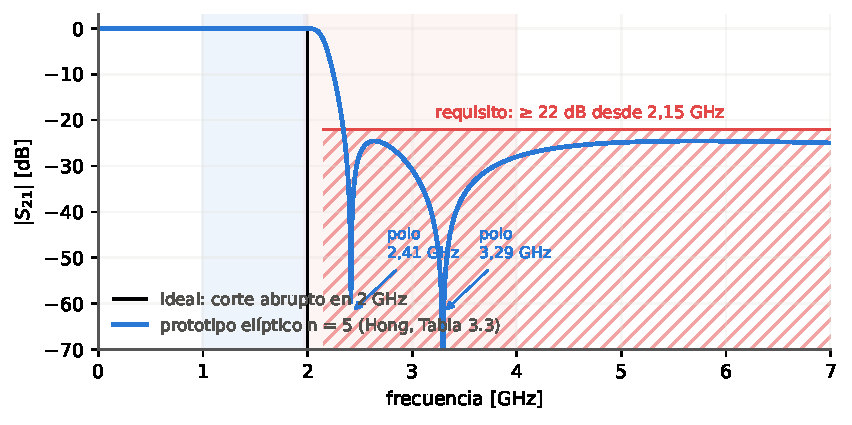
\includegraphics[width=\linewidth]{figuras/filtro_rf/buscado.pdf}
  \caption{Lo que se busca. En negro, el filtro ideal con corte abrupto en
  $2\,\text{GHz}$. En rojo rayado, la zona que pide el requisito
  ($\geq 22\,\text{dB}$ desde $2{,}15\,\text{GHz}$). En azul, la
  transferencia teórica del prototipo elíptico de orden 5 que se usó (Hong,
  Tabla~3.3), con sus dos polos. En celeste la banda del VCO y en rosa el
  segundo armónico.}
  \label{fig:frf_buscado}
\end{figure}

%------------------------------------------------------------
\section{Restricciones y especificación}
\label{sec:frf_spec}

El filtro tiene que poder hacerse en una placa común, sin componentes:
\begin{itemize}
  \item \textbf{FR4 de $1{,}6\,\text{mm}$, bifaz.} Los laminados de RF (Rogers)
    no se consiguen en Argentina. Arriba van las pistas y abajo un plano de
    masa entero, que es justo lo que necesita un microstrip. Se eligió
    $1{,}6\,\text{mm}$ porque las pistas salen más anchas y el error del
    fabricante pesa menos en porcentaje.
  \item \textbf{$\varepsilon_r$ desconocido.} El FR4 es genérico y el
    fabricante no informa su $\varepsilon_r$. Se diseñó con $4{,}4$ y se
    consideró un rango de $4{,}2$ a $4{,}8$.
  \item \textbf{Peor tolerancia.} Ancho de pista $\pm 0{,}15\,\text{mm}$ y
    espesor $\pm 10$\,\%.
  \item \textbf{Conectores SMA} y nada más que pistas de cobre.
\end{itemize}

\begin{table}[htbp]
  \centering
  \caption{Especificación con la que se diseñó.}
  \label{tab:frf_spec}
  \begin{tabular}{ll}
    \toprule
    Borde de la banda de paso & $f_c = 2{,}05\,\text{GHz}$, rizado $0{,}1\,\text{dB}$ \\
    Comienzo del rechazo & $f_s = 2{,}356\,\text{GHz}$ ($\Omega_s = 1{,}1494$) \\
    Atenuación mínima teórica & $24{,}5\,\text{dB}$ ($n = 5$), $45{,}7\,\text{dB}$ ($n = 7$) \\
    Rechazo hasta & al menos $4\,\text{GHz}$ (ideal $6\,\text{GHz}$, tercer armónico) \\
    Impedancia & $50\,\Omega$ \\
    \bottomrule
  \end{tabular}
\end{table}

El margen entre $2\,\text{GHz}$ y $f_c = 2{,}05\,\text{GHz}$ cubre la
incertidumbre del $\varepsilon_r$. El comienzo del rechazo quedó en
$2{,}356\,\text{GHz}$, que es la fila de la tabla del libro más cercana a
lo buscado. Es más arriba que los $2{,}15\,\text{GHz}$ del requisito, y se
discute en la Sección~\ref{sec:frf_resultado}.

%------------------------------------------------------------
\section{Topología y método}
\label{sec:frf_metodo}

Se eligió un \textbf{pasabajos elíptico en microstrip de impedancia
escalonada con stubs resonantes}, y se siguió al pie de la letra el
procedimiento de Hong y Lancaster \cite{Hong2001}, Sección~5.1.3
(\emph{Semilumped lowpass filters having finite-frequency attenuation
poles}). El prototipo es una escalera (Figura~\ref{fig:frf_escalera}):
\begin{itemize}
  \item las \textbf{L en serie} ($g_1$, $g_3$, $g_5$) se hacen con
    \textbf{tramos finos} de alta impedancia,
  \item cada \textbf{rama L--C a masa} ($g_i'$ en serie con $g_i$) se hace con
    un \textbf{stub}, o sea un tramo fino (la L) que termina en un parche ancho
    con el extremo abierto (la C contra el plano de masa). En la frecuencia en que
    la rama resuena, el stub es un cortocircuito a masa y la transmisión cae a
    cero. Ése es el \emph{polo}, en
    $\Omega = 1/\sqrt{g_i\,g_i'}$.
\end{itemize}

\begin{figure}[htbp]
  \centering
  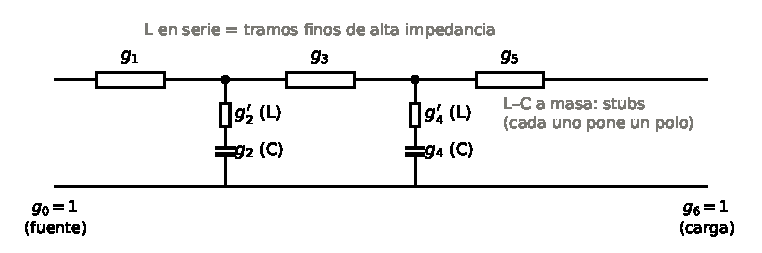
\includegraphics[width=\linewidth]{figuras/filtro_rf/escalera.pdf}
  \caption{Prototipo elíptico de orden 5 (Hong, Figura~3.11b).}
  \label{fig:frf_escalera}
\end{figure}

Se hicieron dos diseños con el mismo método, \textbf{A} de orden 5 (dos
polos) y \textbf{B} de orden 7 (tres polos).

%------------------------------------------------------------
\section{Diseño paso a paso}
\label{sec:frf_diseno}

Todo el cálculo está en \texttt{GPRv2/\allowbreak docs/\allowbreak FILTRO\_RF/\allowbreak diseno\_hong.py},
que cita en cada paso la ecuación del libro y escribe los resultados en
\texttt{diseno\_hong.json}. Para comprobar que se usan las ecuaciones igual
que el libro, el script reproduce el ejemplo de la Sección~5.1.3: da
$\ell_{L2} = 2{,}96\,\text{mm}$ y $\ell_{C2} = 5{,}62\,\text{mm}$, contra
$2{,}98$ y $5{,}61\,\text{mm}$ del libro (la diferencia es que el libro
redondea $\lambda_g$ a milímetros enteros).

\subsection{Prototipo}

Los valores salen de la Tabla~3.3 de Hong, hecha para rizado
$L_{Ar} = 0{,}1\,\text{dB}$ y $g_0 = g_{n+1} = 1$. Se normaliza
$\Omega_s = f_s/f_c$ y se toma la fila correspondiente
(Tabla~\ref{tab:frf_g}).

\begin{table}[htbp]
  \centering
  \caption{Valores del prototipo usados (Hong, Tabla~3.3, $\Omega_s = 1{,}1494$).}
  \label{tab:frf_g}
  \small
  \resizebox{\linewidth}{!}{%
  \begin{tabular}{lcccccccccc}
    \toprule
    & $g_1$ & $g_2$ & $g_2'$ & $g_3$ & $g_4$ & $g_4'$ & $g_5$ & $g_6$ & $g_6'$ & $g_7$ \\
    \midrule
    A ($n=5$) & 0,8726 & 1,0084 & 0,3845 & 1,3097 & 0,4991 & 1,4450 & 0,4302 & & & \\
    B ($n=7$) & 1,0252 & 1,2157 & 0,1940 & 1,5811 & 0,9939 & 0,5816 & 1,2382 & 0,5243 & 1,4096$^*$ & 0,4369 \\
    \bottomrule
  \end{tabular}}
\end{table}

\paragraph{Errata de la Tabla~3.3.} ($^*$) En $n = 7$ la columna $g_6'$ del
libro repite los valores de $g_4'$ en todas las filas. Con el valor impreso
($0{,}5816$) el polo cae en $\Omega = 1{,}811$, que no es un cero de la
función elíptica. Sintetizando el prototipo se obtiene $g_6' = 1{,}4096$, y
con ese valor el polo cae en $\Omega = 1{,}1633$, que sí lo es. Se encontró
verificando los polos, que conviene hacer siempre.

\subsection{Escalado}

Para $Z_0 = 50\,\Omega$ y $\omega_c = 2\pi f_c$ (ecuación~5.6 del libro):
\begin{equation}
  L = \frac{g\,Z_0}{\omega_c} = g \cdot 3{,}882\,\text{nH}, \qquad
  C = \frac{g}{Z_0\,\omega_c} = g \cdot 1{,}553\,\text{pF},
\end{equation}
y cada rama pone un polo en $f_p = 1/(2\pi\sqrt{L'C})$ (ecuación~5.8).

\begin{table}[htbp]
  \centering
  \caption{Valores escalados. Los stubs van numerados de la entrada a la salida.}
  \label{tab:frf_escalado}
  \resizebox{\linewidth}{!}{%
  \begin{tabular}{lll}
    \toprule
    & A ($n = 5$) & B ($n = 7$) \\
    \midrule
    L en serie & 3,39 / 5,08 / 1,67 nH & 3,98 / 6,14 / 4,81 / 1,70 nH \\
    Stub 1: $C$ / $L'$ / polo & 1,57 pF / 1,49 nH / 3,29 GHz & 1,89 pF / 0,753 nH / 4,22 GHz \\
    Stub 2: $C$ / $L'$ / polo & 0,775 pF / 5,61 nH / 2,41 GHz & 1,54 pF / 2,26 nH / 2,70 GHz \\
    Stub 3: $C$ / $L'$ / polo & & 0,814 pF / 5,47 nH / 2,39 GHz \\
    \bottomrule
  \end{tabular}}
\end{table}

\subsection{Impedancias de las líneas}

El ancho de cada línea sale de las fórmulas de Hammerstad y Jensen
(ecuaciones~4.4 y 4.5 del libro), con $\varepsilon_r = 4{,}4$ y
$h = 1{,}6\,\text{mm}$. Hay que elegir la impedancia alta $Z_{0L}$ (tramos
finos) y la baja $Z_{0C}$ (parches). El libro da los criterios. Con $Z_{0L}$
más alta la línea se parece más a una L ideal, pero es más fina y difícil de
fabricar. Con $Z_{0C}$ más baja el parche se parece más a una C ideal, pero se
ensancha y puede resonar a lo ancho.

Se eligió con la peor tolerancia. Para cada combinación se armó el filtro
con líneas de transmisión, se ajustaron los largos al prototipo y se evaluaron
las 8 esquinas de ancho $\pm 0{,}15\,\text{mm}$, $\varepsilon_r$ de $4{,}2$ a
$4{,}8$ y espesor $\pm 10$\,\% (Tabla~\ref{tab:frf_tolerancias}).

\begin{table}[htbp]
  \centering
  \caption{Elección de impedancias con peor tolerancia (diseño A, modelo de
  líneas ideales, sin discontinuidades).}
  \label{tab:frf_tolerancias}
  \begin{tabular}{cccc}
    \toprule
    $Z_{0L}$ / $Z_{0C}$ & rechazo nominal & rechazo peor caso & reapertura $> 4\,\text{GHz}$, peor caso \\
    \midrule
    90 / 25 $\Omega$  & $-12\,\text{dB}$ & $-8\,\text{dB}$ & $\sim 0\,\text{dB}$ \\
    100 / 25 $\Omega$ & $-16{,}5\,\text{dB}$ & $-10{,}5\,\text{dB}$ & $-2\,\text{dB}$ \\
    110 / 25 $\Omega$ & $-20{,}5\,\text{dB}$ & $-13{,}4\,\text{dB}$ & $-5\,\text{dB}$ \\
    \textbf{110 / 30 $\Omega$} & $\mathbf{-20{,}4\,dB}$ & $\mathbf{-13{,}8\,dB}$ & $\mathbf{-5\,dB}$ \\
    \bottomrule
  \end{tabular}
\end{table}

Quedó $Z_{0L} = 110\,\Omega$ ($0{,}536\,\text{mm}$) y $Z_{0C} = 30\,\Omega$
($6{,}577\,\text{mm}$). La línea de $50\,\Omega$ mide $3{,}066\,\text{mm}$.
La conclusión importante es que \textbf{la tolerancia que manda es el
$\varepsilon_r$, no el ancho}. $\pm 0{,}15\,\text{mm}$ de ancho mueve el
rechazo menos de $0{,}5\,\text{dB}$, porque la inductancia la fija sobre todo
el largo de la pista y el grabado no cambia el largo. En cambio, pasar de
$\varepsilon_r = 4{,}2$ a $4{,}8$ corre los polos $\pm 3$\,\% y empeora el
rechazo unos $4\,\text{dB}$.

En el diseño B el parche quedó en $Z_{0C} = 20\,\Omega$
($11{,}11\,\text{mm}$). Con $30\,\Omega$ el stub 1 (el de $4{,}22\,\text{GHz}$,
que pide mucha C y poca L) daba un tramo fino de largo negativo. Se siguió el
criterio del libro de bajar $Z_{0C}$.

\subsection{Largos}

Cada L y cada C se pasa a un tramo de línea con la ecuación~5.9:
\begin{equation}
  \ell_L = \frac{\lambda_{gL}}{2\pi}\,\sin^{-1}\!\left(\frac{\omega_c L}{Z_{0L}}\right),
  \qquad
  \ell_C = \frac{\lambda_{gC}}{2\pi}\,\sin^{-1}\!\left(\omega_c Z_{0C}\, C\right),
\end{equation}
con $\lambda_g$ de la ecuación~4.6b. Después se aplican dos correcciones:
\begin{itemize}
  \item \textbf{Uniones} (ecuación~5.11). Las puntas de los tramos finos que
    llegan a cada unión agregan una susceptancia $\Delta B_{123}$. Se pide que
    el stub real más esa susceptancia se comporte como la rama L--C, y se
    resuelve en $f_c$ y en el polo de cada stub. Son dos ecuaciones y dos
    incógnitas por stub (el largo del tramo fino y el del parche). Los tramos
    en serie no se tocan, igual que en el libro. La ecuación~5.10 no aplica,
    porque corrige una C final que los prototipos de orden impar no tienen.
  \item \textbf{Extremo abierto} (ecuación~4.40). El campo se escapa por la
    punta del parche, que se ve más largo de lo que es. Se le resta $\Delta
    \ell$: $0{,}755\,\text{mm}$ en A y $0{,}812\,\text{mm}$ en B.
\end{itemize}

\paragraph{Errata de la ecuación~4.40.} El factor $\xi_1$ aparece impreso como
un solo cociente. En la fórmula original (Kirschning, Jansen y Koster) es un
producto,
\begin{equation*}
  \xi_1 = 0{,}434907\,
  \frac{\varepsilon_{re}^{0{,}81} + 0{,}26}{\varepsilon_{re}^{0{,}81} - 0{,}189}
  \cdot
  \frac{u^{0{,}8544} + 0{,}236}{u^{0{,}8544} + 0{,}87}.
\end{equation*}
Con la versión impresa el ejemplo del libro da $\Delta\ell = 0{,}71\,\text{mm}$.
Con ésta da $0{,}535\,\text{mm}$, que es el $0{,}54\,\text{mm}$ que usa el
propio libro.

\begin{table}[htbp]
  \centering
  \caption{Largos de los stubs en mm (tramo fino / parche). Inicial según la
  ec.~5.9, corregido según la ec.~5.11 y final con el $\Delta\ell$ del parche restado.}
  \label{tab:frf_largos}
  \begin{tabular}{llccc}
    \toprule
    & stub (polo) & inicial & corregido & final \\
    \midrule
    A & 1 (3,29 GHz) & 2,36 / 8,01 & 1,04 / 8,66 & 1,04 / 7,91 \\
      & 2 (2,41 GHz) & 9,63 / 3,75 & 8,09 / 3,12 & 8,09 / 2,36 \\
    \midrule
    B & 1 (4,22 GHz) & 1,19 / 6,11 & 0,44 / 7,06 & 0,44 / 6,25 \\
      & 2 (2,70 GHz) & 3,60 / 4,92 & 2,72 / 5,31 & 2,72 / 4,50 \\
      & 3 (2,39 GHz) & 9,35 / 2,54 & 8,35 / 2,07 & 8,35 / 1,26 \\
    \bottomrule
  \end{tabular}
\end{table}

Los tramos en serie miden $5{,}48$, $8{,}57$ y $2{,}65\,\text{mm}$ en A, y
$6{,}52$, $10{,}78$, $8{,}03$ y $2{,}69\,\text{mm}$ en B.

\subsection{Geometría final}

La Figura~\ref{fig:frf_topologias} muestra los dos diseños. En B los parches
miden $11{,}1\,\text{mm}$ de ancho y los stubs están separados $10{,}8$ y
$8{,}0\,\text{mm}$, así que del mismo lado se pisarían. Por eso el del medio
va del otro lado de la línea. El libro no trata este caso.

\begin{figure}[htbp]
  \centering
  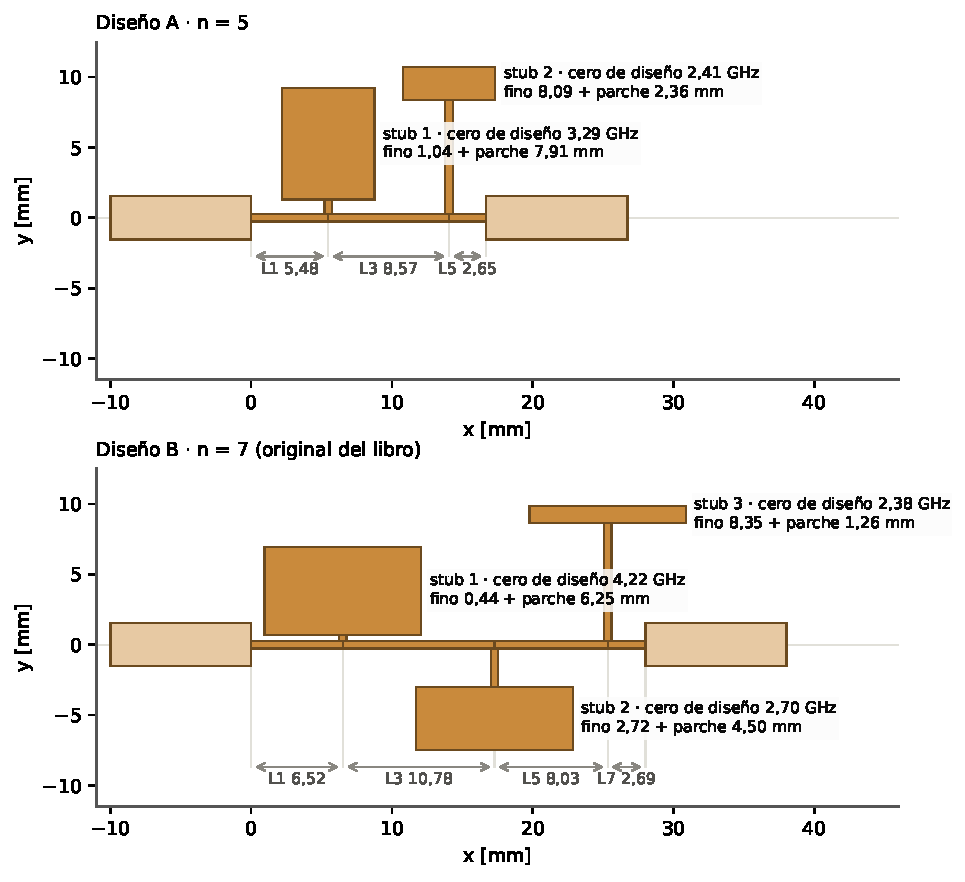
\includegraphics[width=\linewidth]{figuras/filtro_rf/topologias.pdf}
  \caption{Geometría de los diseños A y B (vista superior, medidas en mm).
  El filtro en cobre oscuro y las líneas de $50\,\Omega$ de los puertos en
  cobre claro.}
  \label{fig:frf_topologias}
\end{figure}

%------------------------------------------------------------
\section{Verificación electromagnética}
\label{sec:frf_em}

El libro cierra el procedimiento con una simulación electromagnética de onda
completa, que ve lo que las fórmulas no ven, como el acople entre parches,
los escalones, las resonancias a lo ancho y la reapertura del filtro a
frecuencias altas. Se usó \textbf{openEMS} \cite{openEMS}, un simulador FDTD libre, que
funciona como el \emph{transient solver} de CST. Los scripts y los resultados
están en \texttt{GPRv2/\allowbreak docs/\allowbreak FILTRO\_RF/\allowbreak openems/}, y
\texttt{dashboard.html} reúne todas las corridas con su modelo, malla, bordes
y puertos tal como los recibió el simulador.

\subsection{Modelo}

\begin{table}[htbp]
  \centering
  \caption{Modelo en openEMS.}
  \label{tab:frf_modelo}
  \begin{tabular}{ll}
    \toprule
    Método & FDTD (dominio del tiempo), una corrida da todo el rango \\
    Excitación & pulso gaussiano de $1$ a $7{,}5\,\text{GHz}$ (a $-20\,\text{dB}$) \\
    Fin de la corrida & energía a $-50\,\text{dB}$, o si se estanca \\
    Masa & borde conductor perfecto debajo del sustrato \\
    Bordes & PML en las puntas de las líneas, MUR a los costados y arriba \\
    Puertos & microstrip de $50\,\Omega$, $10\,\text{mm}$, terminados en $50\,\Omega$ \\
    Referencia & corrida hasta el borde del filtro \\
    Malla & $\lambda/20$ a $7\,\text{GHz}$ ($\sim\!1\,\text{mm}$), $0{,}045$ a $0{,}13\,\text{mm}$ en los bordes \\
    Sustrato & FR4, $\varepsilon_r = 4{,}4$, $h = 1{,}6\,\text{mm}$ \\
    Conductor & PEC, cobre en lámina o cobre de $72\,\mu\text{m}$ en bloque \\
    \bottomrule
  \end{tabular}
\end{table}

\begin{figure}[htbp]
  \centering
  \begin{subfigure}{0.62\linewidth}
    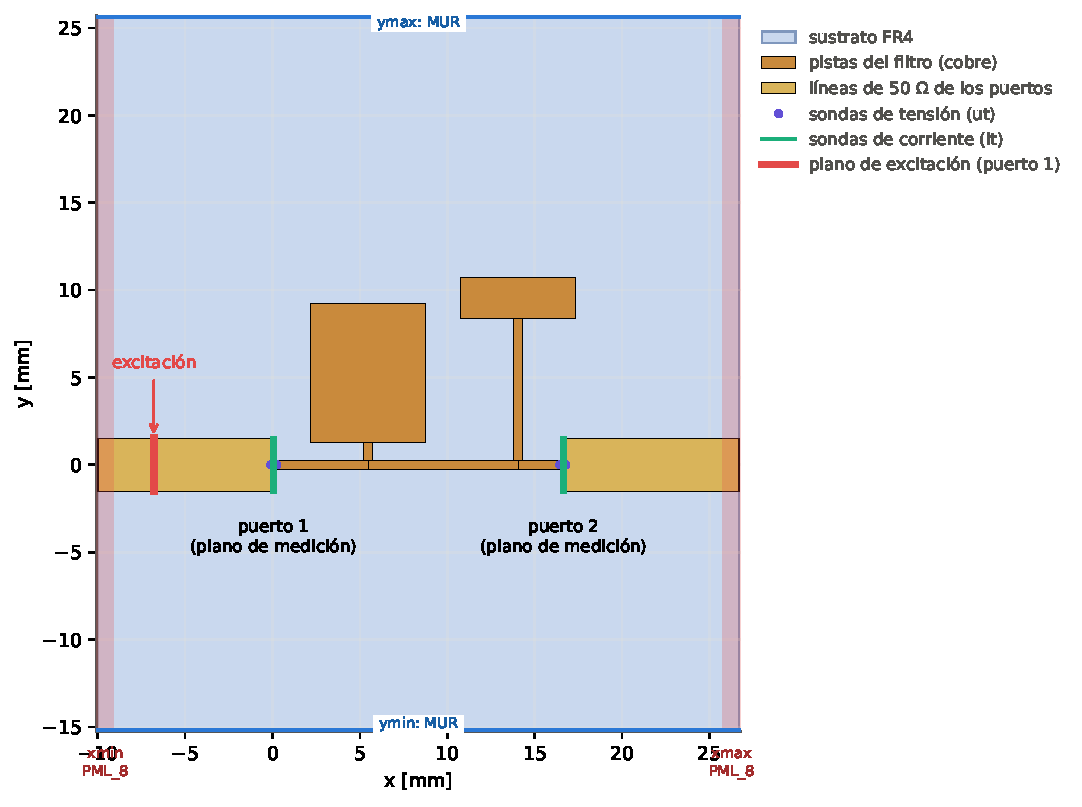
\includegraphics[width=\linewidth]{figuras/filtro_rf/modelo_topologia.pdf}
    \caption{Vista superior con sustrato, pistas, puertos y bordes.}
  \end{subfigure}
  \begin{subfigure}{\linewidth}
    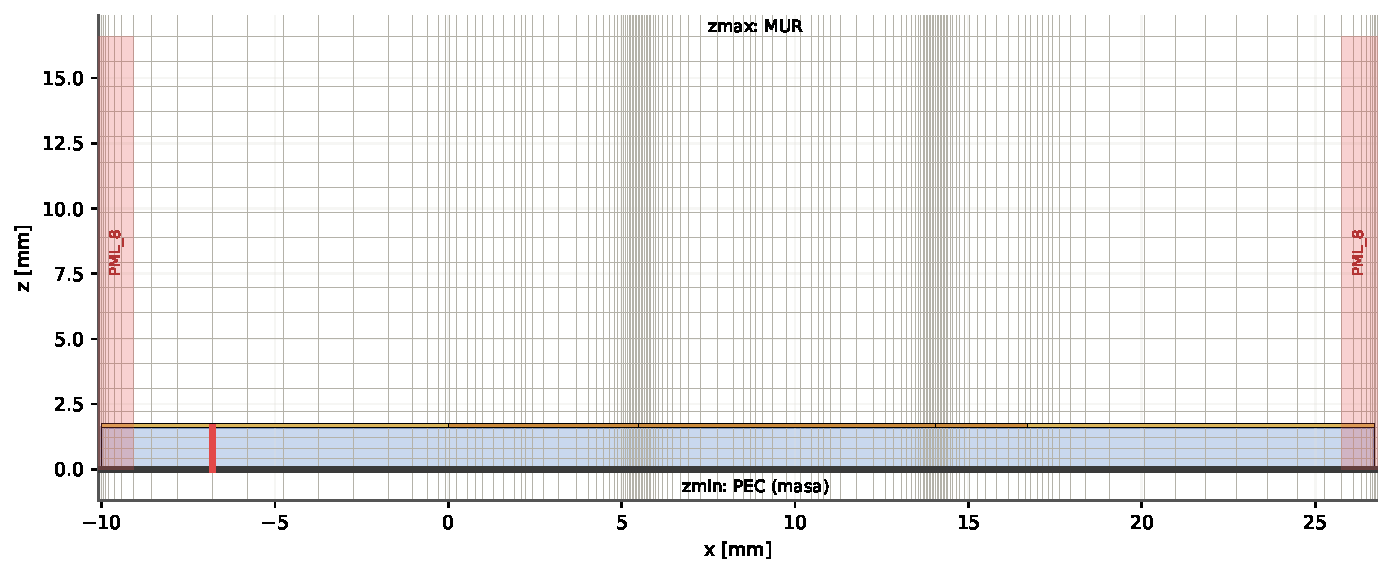
\includegraphics[width=\linewidth]{figuras/filtro_rf/modelo_corte.pdf}
    \caption{Corte lateral con la malla. El metal está en $z = h$.}
  \end{subfigure}
  \caption{Modelo del diseño A, dibujado a partir del archivo que recibe el
  simulador.}
  \label{fig:frf_modelo}
\end{figure}

\subsection{Convergencia de malla}

Se corrió el diseño A sin pérdidas con tres mallas
(Tabla~\ref{tab:frf_convergencia} y Figura~\ref{fig:frf_convergencia}).

\begin{table}[htbp]
  \centering
  \caption{Convergencia de malla (diseño A, PEC).}
  \label{tab:frf_convergencia}
  \resizebox{\linewidth}{!}{%
  \begin{tabular}{lcccc}
    \toprule
    malla & celdas / tiempo & borde $-1\,\text{dB}$ & polos & atenuación mín. $2{,}36$--$4\,\text{GHz}$ \\
    \midrule
    $\lambda/20$ & 0,35 M / 3,4 min & 2,051 GHz & 2,482 / 3,679 GHz & 19,0 dB \\
    $\lambda/30$ & 0,56 M / 4,7 min & 2,046 GHz & 2,482 / 3,674 GHz & 19,3 dB \\
    $\lambda/40$ & 0,90 M / 6,0 min & 2,036 GHz & 2,468 / 3,649 GHz & 21,0 dB \\
    \bottomrule
  \end{tabular}}
\end{table}

\begin{figure}[htbp]
  \centering
  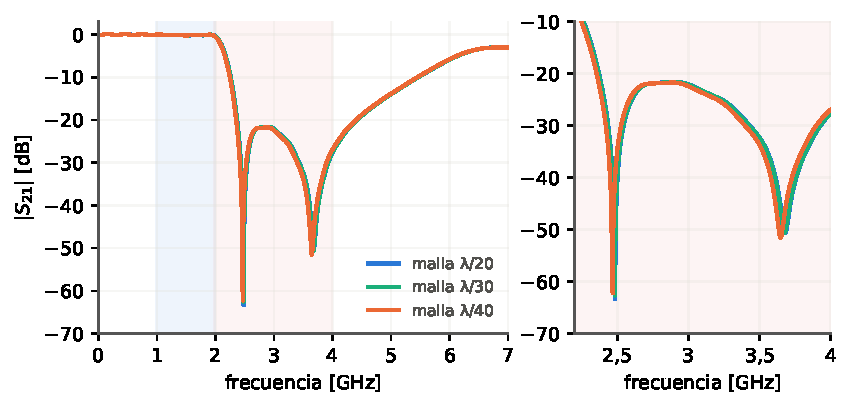
\includegraphics[width=\linewidth]{figuras/filtro_rf/convergencia.pdf}
  \caption{Convergencia de malla del diseño A. A la derecha, zoom en la zona
  de los polos.}
  \label{fig:frf_convergencia}
\end{figure}

De $\lambda/20$ a $\lambda/40$ los polos se mueven menos del $1$\,\% y el
rechazo unos $2\,\text{dB}$. Es bastante menos que lo que mueve la
tolerancia del $\varepsilon_r$, así que \textbf{todo lo demás se corrió en
$\lambda/20$}.

\subsection{Diseños A y B contra el prototipo}

\begin{figure}[htbp]
  \centering
  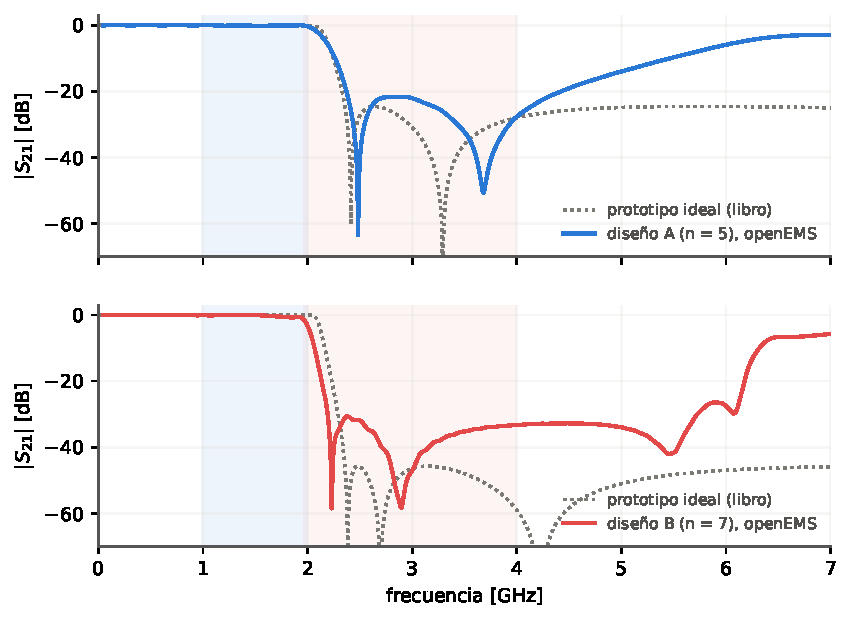
\includegraphics[width=\linewidth]{figuras/filtro_rf/pec_contra_prototipo.pdf}
  \caption{Diseños A y B simulados (PEC, sin pérdidas) contra su prototipo
  ideal.}
  \label{fig:frf_pec}
\end{figure}

\paragraph{Diseño A.} La banda de paso funciona. El borde de $-1\,\text{dB}$
cae en $2{,}05\,\text{GHz}$, la pérdida no pasa de $0{,}32\,\text{dB}$ y
$|S_{11}| \leq -11\,\text{dB}$. El polo de $2{,}41\,\text{GHz}$ cae casi justo
($2{,}48\,\text{GHz}$, $+3$\,\%), porque ese stub (tramo fino largo y parche
chico) se parece mucho a la rama ideal. El de $3{,}29\,\text{GHz}$ se corre a
$3{,}68\,\text{GHz}$ ($+12$\,\%). Ese stub es casi todo parche y ahí el
modelo de L y C concentradas deja de valer. Por eso el rechazo mínimo queda en
$19\,\text{dB}$ en vez de los $24{,}5$ del prototipo. Arriba de
$\sim\!4{,}5\,\text{GHz}$ el filtro vuelve a dejar pasar ($-3\,\text{dB}$
cerca de $7\,\text{GHz}$). Es el pico espurio que muestra el propio libro en
su Figura~5.7.

\paragraph{Diseño B.} Rechaza mucho mejor ($30{,}6\,\text{dB}$ en todo el
segundo armónico y $\sim\!-33\,\text{dB}$ hasta $5{,}5\,\text{GHz}$), pero toda
la curva quedó corrida hacia abajo. El primer polo cayó en $2{,}23\,\text{GHz}$
contra $2{,}39$ de diseño ($-7$\,\%), y con él el borde de la banda de paso, que
pierde $3{,}2\,\text{dB}$ en $2\,\text{GHz}$. La explicación más probable es
que los parches de $11\,\text{mm}$ de ancho ya no se comportan como
capacitores concentrados y se ven eléctricamente más largos.

\subsection{Ajuste del diseño B}

Como cierre del diseño con la simulación, se acortaron todos los stubs de B
(tramo fino y parche) por $2{,}229/2{,}385 = 0{,}935$, el cociente entre el
polo simulado y el de diseño. Como la frecuencia de resonancia es inversa al
largo, eso corre todo hacia arriba en la misma proporción
(Figura~\ref{fig:frf_recorte}).

\begin{figure}[htbp]
  \centering
  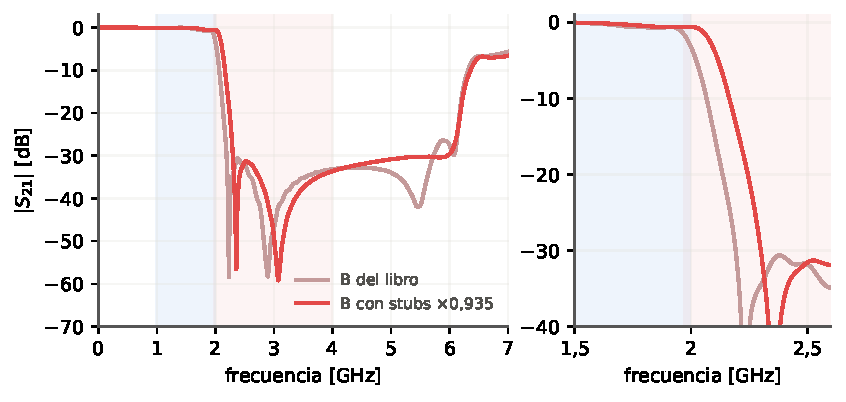
\includegraphics[width=\linewidth]{figuras/filtro_rf/recorte_B.pdf}
  \caption{Diseño B tal como sale del libro y con los stubs acortados
  $\times 0{,}935$ (PEC). A la derecha, zoom en el borde de la banda.}
  \label{fig:frf_recorte}
\end{figure}

El borde volvió a $2{,}05\,\text{GHz}$, la pérdida en $2\,\text{GHz}$ bajó de
$3{,}2$ a $0{,}6\,\text{dB}$, $|S_{11}|$ en la banda pasó de $-4$ a
$-9\,\text{dB}$, y el rechazo quedó igual ($31\,\text{dB}$). De acá en
adelante el diseño B es el recortado.

\subsection{Pérdidas y espesor del cobre}

Se compararon tres modelos de conductor: PEC sin pérdidas, cobre en lámina
($\sigma = 5{,}8\cdot 10^7\,\text{S/m}$, los $72\,\mu\text{m}$ sólo cuentan para
las pérdidas) y cobre de $72\,\mu\text{m}$ en bloque, que es lo más parecido a
CST. Con cobre, el FR4 también tiene pérdidas, con $\tan\delta = 0{,}025$ como
el FR-4 de la biblioteca de CST. openEMS modela esa pérdida como una
conductividad fija, así que se clavó en $2{,}05\,\text{GHz}$ y varía como
$1/f$.

\begin{figure}[htbp]
  \centering
  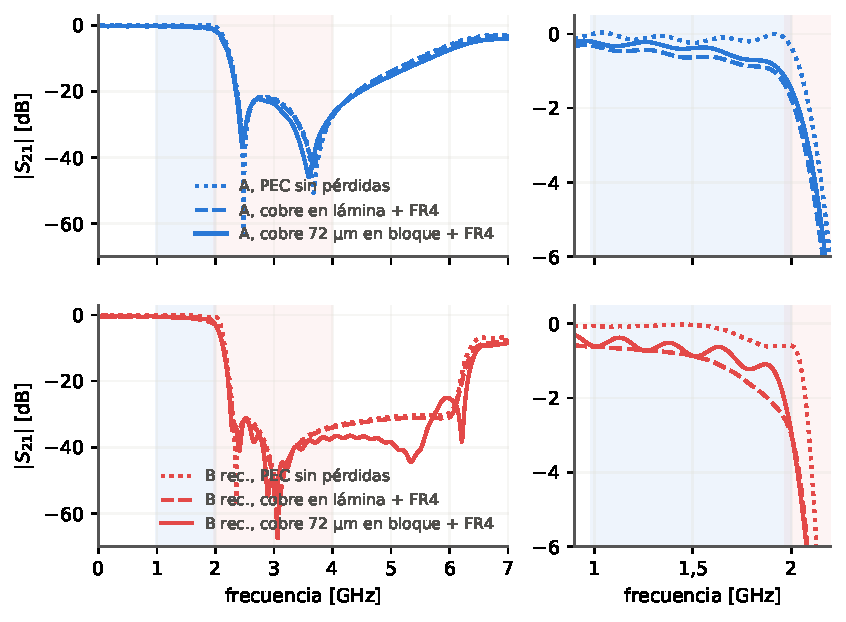
\includegraphics[width=\linewidth]{figuras/filtro_rf/conductor.pdf}
  \caption{Modelo del conductor, arriba A y abajo B recortado. A la derecha,
  zoom en la banda de paso.}
  \label{fig:frf_conductor}
\end{figure}

\begin{table}[htbp]
  \centering
  \caption{Modelo del conductor ($\lambda/20$). $|S_{21}|$ en dB.}
  \label{tab:frf_conductor}
  \small
  \resizebox{\linewidth}{!}{%
  \begin{tabular}{lcccccc}
    \toprule
    & A PEC & A lámina & A bloque & B PEC & B lámina & B bloque \\
    \midrule
    $|S_{21}|$ en 1,0 / 1,5 GHz & 0 / $-0{,}25$ & $-0{,}33$ / $-0{,}64$ & $-0{,}22$ / $-0{,}38$ & $-0{,}06$ / $-0{,}04$ & $-0{,}62$ / $-0{,}87$ & $-0{,}61$ / $-0{,}87$ \\
    $|S_{21}|$ en 1,9 / 2,0 GHz & $-0{,}02$ / $-0{,}36$ & $-0{,}97$ / $-1{,}75$ & $-0{,}80$ / $-1{,}48$ & $-0{,}61$ / $-0{,}59$ & $-2{,}1$ / $-3{,}0$ & $-1{,}2$ / $-2{,}9$ \\
    polos [GHz] & 2,48 / 3,68 & 2,47 / 3,68 & 2,46 / 3,60 & 2,35 / 3,07 & 2,35 / 3,06 & 2,41 / 3,03 \\
    rechazo mín. 2,36--4 GHz & 19,0 & 20,3 & 21,5 & 31,3 & 32,0 & 31,1 \\
    \bottomrule
  \end{tabular}}
\end{table}

Las pérdidas no mueven los polos, los hacen menos profundos, y suman entre
$0{,}2$ y $3\,\text{dB}$ de pérdida en la banda del VCO, casi toda del FR4. El
cobre en bloque pierde $0{,}1$ a $0{,}3\,\text{dB}$ menos que la lámina y baja
los polos un $1$ a $2$\,\%. Para este filtro la lámina alcanza.

\subsection{Confirmación con MEEP}

Se simularon A y B también con MEEP \cite{Oskooi2010}, otro programa FDTD,
como control independiente. MEEP sólo admite una malla uniforme, y a
$8\,\text{px/mm}$ (celdas de $0{,}125\,\text{mm}$) cada diseño ya tardó entre
$40$ y $76$ minutos con 6 procesos. Con esa malla la línea fina queda con
apenas 4 celdas y todo se redondea a múltiplos de $0{,}125\,\text{mm}$. Además
MEEP no tiene puertos microstrip. La señal se inyecta con una fuente de
campo y los parámetros S salen de flujos de potencia.

\begin{figure}[htbp]
  \centering
  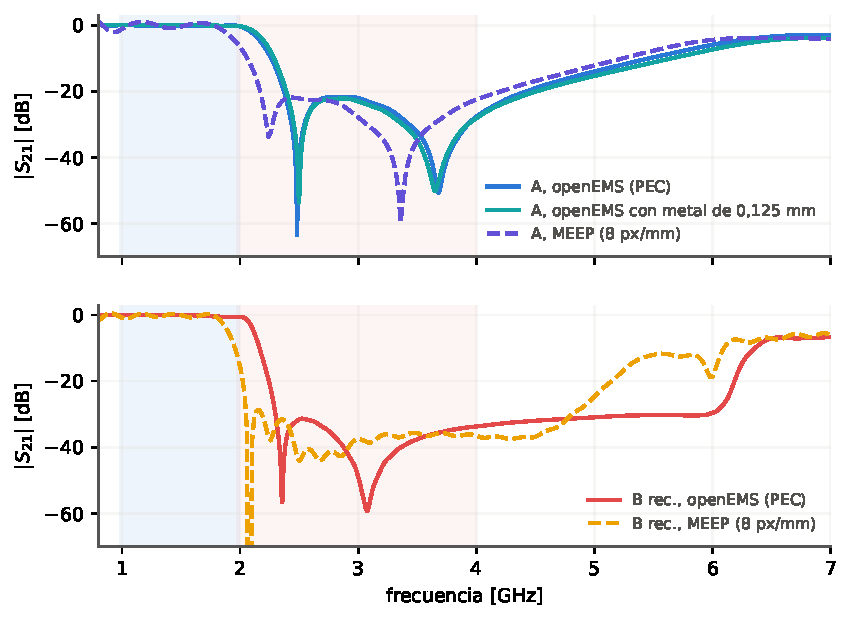
\includegraphics[width=\linewidth]{figuras/filtro_rf/meep.pdf}
  \caption{openEMS contra MEEP, sin pérdidas. Arriba A (con el control de
  metal de $0{,}125\,\text{mm}$), abajo B recortado.}
  \label{fig:frf_meep}
\end{figure}

MEEP ve la misma forma (los polos, el nivel de rechazo, la reapertura), pero
corre toda la respuesta $\sim\!10$\,\% hacia abajo. Se descartó que fuera por
el espesor del metal (en MEEP ocupa una celda, $0{,}125\,\text{mm}$):
simulando A en openEMS con metal de ese espesor los polos se mueven menos de
$1$\,\%. Afinar la malla de MEEP llevaría de 3 a 10 horas por diseño.
\textbf{Los resultados de MEEP sólo sirven para confirmar la topología}, no
como medición precisa. Para las frecuencias manda openEMS, que tiene la malla
refinada en los bordes y su estudio de convergencia.

%------------------------------------------------------------
\section{Resultado contra lo buscado}
\label{sec:frf_resultado}

\begin{figure}[htbp]
  \centering
  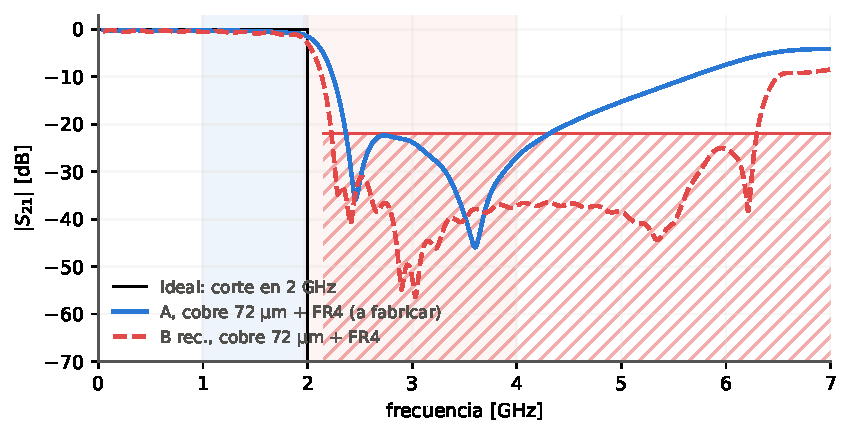
\includegraphics[width=\linewidth]{figuras/filtro_rf/obtenido.pdf}
  \caption{Lo buscado contra lo obtenido. En negro, el filtro ideal. En rojo
  rayado, la zona del requisito. En color, los dos diseños con cobre de
  $72\,\mu\text{m}$ y FR4 con pérdidas.}
  \label{fig:frf_obtenido}
\end{figure}

\begin{table}[htbp]
  \centering
  \caption{Requisitos contra los diseños (cobre de $72\,\mu\text{m}$ y FR4 con
  pérdidas).}
  \label{tab:frf_resultado}
  \begin{tabular}{lcc}
    \toprule
    & A & B recortado \\
    \midrule
    Pérdida en la banda del VCO & 0,2 a 1,4 dB & 0,4 a 2,8 dB \\
    $|S_{11}|$ máximo en la banda & $-12{,}4\,\text{dB}$ & $-14{,}0\,\text{dB}$ \\
    $|S_{21}|$ en 2,15 GHz (se pide $\leq -22\,\text{dB}$) & $-5{,}0\,\text{dB}$ & $-11{,}1\,\text{dB}$ \\
    Atenúa 22 dB a partir de & 2,37 GHz & 2,23 GHz \\
    Atenuación mín. 2,36--4 GHz & 21,5 dB & 31,1 dB \\
    $|S_{21}|$ en 4 / 5 / 6 GHz & $-27$ / $-15$ / $-7\,\text{dB}$ & $-37$ / $-38$ / $-25\,\text{dB}$ \\
    \bottomrule
  \end{tabular}
\end{table}

Ninguno llega a los $22\,\text{dB}$ desde $2{,}15\,\text{GHz}$. El diseño se
hizo con el rechazo desde $2{,}36\,\text{GHz}$, y además el filtro real cae más
lento que el prototipo. La consecuencia es que queda más rampa contaminada.
Con la cuenta pesimista de la Sección~\ref{sub:armonicos_requisitos} (banda de
$988$ a $1991\,\text{MHz}$, nada de atenuación por debajo del punto en que se
alcanzan los $22\,\text{dB}$), el fantasma que se cuela por el borde de la
rampa queda en:
\begin{itemize}
  \item \textbf{A} atenúa $22\,\text{dB}$ recién desde $2{,}37\,\text{GHz}$ y
    deja contaminado el $\sim\!20$\,\% de la rampa. Con Hann ese tramo pesa
    $-27\,\text{dB}$ y el fantasma queda en $-50\,\text{dB}$
    ($\Delta G_2 = -7\,\text{dB}$) o $-43\,\text{dB}$ ($\Delta G_2 = 0$).
  \item \textbf{B recortado} los atenúa desde $2{,}23\,\text{GHz}$ y deja el
    $\sim\!13$\,\% de la rampa. Con Hann pesa $-38\,\text{dB}$ y el fantasma
    queda en $-61$ o $-54\,\text{dB}$.
\end{itemize}
Con A el fantasma queda alrededor del piso actual de las capturas
($\sim\!-45\,\text{dB}$), pero no llega al margen de $-60\,\text{dB}$ pensado
para el GPR. Con B sí. A cambio, B pierde $\sim\!1\,\text{dB}$ más en el tope
de la banda. En los dos, la pérdida crece a lo largo de la banda (de $0{,}2$ a
$1{,}4\,\text{dB}$ en A), lo que es una leve modulación de amplitud de la
rampa. Ese tramo cae en el borde de la rampa, donde Hann ya pesa poco.

%------------------------------------------------------------
\section{Se fabrica el diseño A}
\label{sec:frf_decision}

Se decidió \textbf{fabricar sólo el diseño A}. B rechaza más, pero no aporta
tanto para lo que cuesta, y A tiene una ventaja práctica. Al ser de menor
orden su pendiente es más suave, así que los polos se pueden mover (por el
$\varepsilon_r$ real del FR4 o recortando los stubs) sin afectar las
frecuencias útiles de la banda del VCO.

El plan para la placa:
\begin{itemize}
  \item \textbf{Stubs recortables.} Los stubs se dibujan algo más largos que
    lo calculado y se recortan con trincheta mientras se mide $S_{21}$. Al
    acortar un stub su polo sube. Sólo se puede acortar, por eso se arranca
    largo. Falta sacar de la simulación cuántos MHz sube cada polo por
    milímetro recortado.
  \item \textbf{Línea de paso} de $50\,\Omega$ del mismo largo, para medir y
    restar la pérdida de los conectores y la línea.
  \item \textbf{Resonador de prueba} ($\lambda/4$ simple), cuyo polo da el
    $\varepsilon_r$ real de esa tirada de placas. Es la tolerancia que manda,
    y con ese dato se sabe cuánto recortar.
  \item \textbf{Medición} con el \emph{tracking generator} del SSA3032X
    (hasta $3{,}2\,\text{GHz}$) o con el VNA.
\end{itemize}

%------------------------------------------------------------
\section{Problemas de la simulación y cómo se resolvieron}
\label{sec:frf_problemas}

Quedan anotados porque costaron horas y son fáciles de repetir.

\begin{itemize}
  \item \textbf{Una malla con saltos grandes hace diverger la simulación.} La función
    de suavizado de openEMS sólo rellena los huecos grandes y no controla la
    relación entre celdas vecinas. Quedaron celdas de $0{,}045\,\text{mm}$
    pegadas a celdas de $0{,}86\,\text{mm}$ (salto $\times 19$). En el diseño
    B la señal de los puertos, en vez de apagarse, empezó a crecer
    $\times 10$ cada $20\,\text{ns}$, y se perdieron 5 horas. Se reemplazó por
    un suavizado propio que limita el salto a $\times 1{,}5$, y el script no
    corre si se pasa.
  \item \textbf{La continua del pulso no deja terminar la simulación.} El pulso de
    $0$ a $7\,\text{GHz}$ trae componente de continua, que queda atrapada como
    campo estático y no se va por ningún borde. La energía se quedaba fija en
    $-30\,\text{dB}$. Terminar los puertos en $50\,\Omega$ no alcanzó. Se
    resolvió con un pulso de $1$ a $7{,}5\,\text{GHz}$, cuya continua está
    $13\,\text{dB}$ más abajo. A $500\,\text{MHz}$ ese pulso todavía está a
    $-26\,\text{dB}$, que sobra para calcular un cociente como $S_{21}$.
  \item \textbf{Cortar en $-40\,\text{dB}$ es poco.} Cortando ahí, dos
    corridas iguales con distinto pulso diferían $0{,}2$ a $0{,}4\,\text{dB}$ en
    $S_{21}$ y hasta $20\,\text{dB}$ en $S_{11}$ por debajo de
    $1{,}5\,\text{GHz}$. Cortando en $-50\,\text{dB}$ coinciden en
    $0{,}04\,\text{dB}$ (Figura~\ref{fig:frf_criterio}). Se pasó a
    $-50\,\text{dB}$, y si la energía no baja $0{,}5\,\text{dB}$ en 2 minutos
    la corrida se corta sola y se usa lo que hay. El diseño B siempre se
    estanca entre $-37$ y $-44\,\text{dB}$.
\end{itemize}

\begin{figure}[htbp]
  \centering
  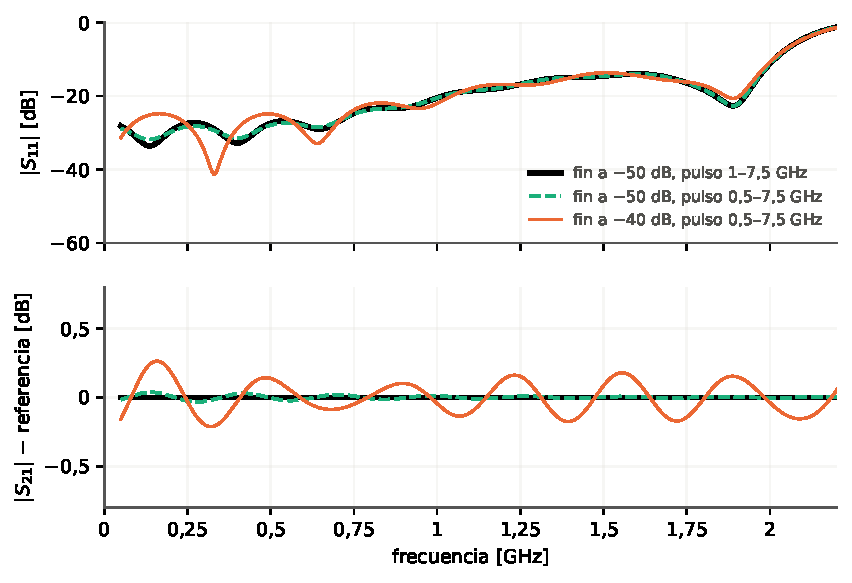
\includegraphics[width=\linewidth]{figuras/filtro_rf/criterio_fin.pdf}
  \caption{Diseño A cortando en $-40$ y en $-50\,\text{dB}$. Arriba
  $|S_{11}|$, abajo la diferencia de $|S_{21}|$ contra la referencia
  ($-50\,\text{dB}$, pulso de $1$ a $7{,}5\,\text{GHz}$).}
  \label{fig:frf_criterio}
\end{figure}

%------------------------------------------------------------
\section{Resumen}

\begin{itemize}
  \item Pasabajos elíptico en microstrip, sin componentes, en FR4 de
    $1{,}6\,\text{mm}$, diseñado siguiendo a Hong y Lancaster paso a paso.
    Se encontraron dos erratas en el libro (Tabla~3.3 y ecuación~4.40).
  \item La tolerancia que manda es el $\varepsilon_r$ del FR4, no el ancho de
    pista.
  \item Simulado en openEMS con malla convergida, tres modelos de conductor y
    confirmación cualitativa con MEEP.
  \item A tiene el borde en $2{,}05\,\text{GHz}$, $21\,\text{dB}$ de rechazo
    mínimo en el segundo armónico y $0{,}2$ a $1{,}4\,\text{dB}$ de pérdida con
    FR4. B recortado da $31\,\text{dB}$ de rechazo con $\sim\!1\,\text{dB}$ más
    de pérdida.
  \item Se fabrica A, con stubs recortables, línea de paso y resonador para
    medir el $\varepsilon_r$.
\end{itemize}
